\subsection*{Problema 30}

\textbf{Enunciado:}
Calcular la integral indefinida:
\begin{align*}
\int x^{-4} (1 + x^2)^{-1/2} \, dx
\end{align*}

\textbf{Solución:}
El integrando es un diferencial binomio de la forma:
\begin{align*}
\int x^m (a + b x^n)^p \, dx
\end{align*}
donde $m = -4$, $n = 2$ y $p = -1/2$. Verificamos los exponentes:
\begin{align*}
\dfrac{m + 1}{n} + p &= \dfrac{-4 + 1}{2} - \dfrac{1}{2} \\
&= -\dfrac{3}{2} - \dfrac{1}{2} = -2
\end{align*}
Dado que este valor es un número entero, aplicamos la sustitución sugerida:
\begin{align*}
z^2 = 1 + x^{-2}
\end{align*}

Derivamos ambos lados para hallar el diferencial:
\begin{align*}
2z \, dz &= -2x^{-3} \, dx \\
z \, dz &= -x^{-3} \, dx
\end{align*}

Reescribimos la integral original para adaptarla al cambio de variable:
\begin{align*}
I &= \int x^{-1} (x^{-3}) (1 + x^2)^{-1/2} \, dx \\
&= \int x^{-1} (x^{-3}) x^{-1/2} (x^{-2} + 1)^{-1/2} \, dx
\end{align*}

Utilizamos la relación $x^{-2} = z^2 - 1$ y $x^{-1} = \sqrt{z^2 - 1}$. Sustituyendo:
\begin{align*}
I &= \int (z^2 - 1)^{-1/2} (z) \, (-z \, dz) \\
&= -\int \dfrac{z^2}{\sqrt{z^2 - 1}} \, dz
\end{align*}

Para resolver esta integral, aplicamos integración por partes o identidades hiperbólicas. Usando integración por partes con $u = z$ y $dv = \dfrac{z}{\sqrt{z^2 - 1}} \, dz$:
\begin{align*}
\int \dfrac{z^2}{\sqrt{z^2 - 1}} \, dz &= z \sqrt{z^2 - 1} \\
&\quad - \int \sqrt{z^2 - 1} \, dz
\end{align*}

Recordando la fórmula de integración para la raíz cuadrada:
\begin{align*}
\int &\sqrt{z^2 - 1} \, dz = \dfrac{z}{2}\sqrt{z^2 - 1} \\
&- \dfrac{1}{2}\ln\left|z + \sqrt{z^2 - 1}\right|
\end{align*}

Sustituyendo de regreso en nuestra integral:
\begin{align*}
I &= -\left[ \dfrac{z}{2}\sqrt{z^2 - 1} \right. \\
&\quad \left. + \dfrac{1}{2}\ln\left|z + \sqrt{z^2 - 1}\right| \right] + C
\end{align*}

Regresando a la variable original mediante $z = \sqrt{1 + x^{-2}}$:
\begin{align*}
\sqrt{z^2 - 1} = \sqrt{x^{-2}} = \dfrac{1}{x}
\end{align*}

Sustituyendo estos valores:
\begin{align*}
I &= -\dfrac{\sqrt{1 + x^{-2}}}{2x} \\
&\quad - \dfrac{1}{2}\ln\left|\sqrt{1 + x^{-2}} + \dfrac{1}{x}\right| + C
\end{align*}

Simplificando el resultado final:
\begin{align*}
I &= -\dfrac{\sqrt{x^2 + 1}}{2x^2} \\
&\quad - \dfrac{1}{2}\ln\left|\dfrac{\sqrt{x^2 + 1} + 1}{x}\right| + C
\end{align*}

\begin{figure}[H]
	\centering
	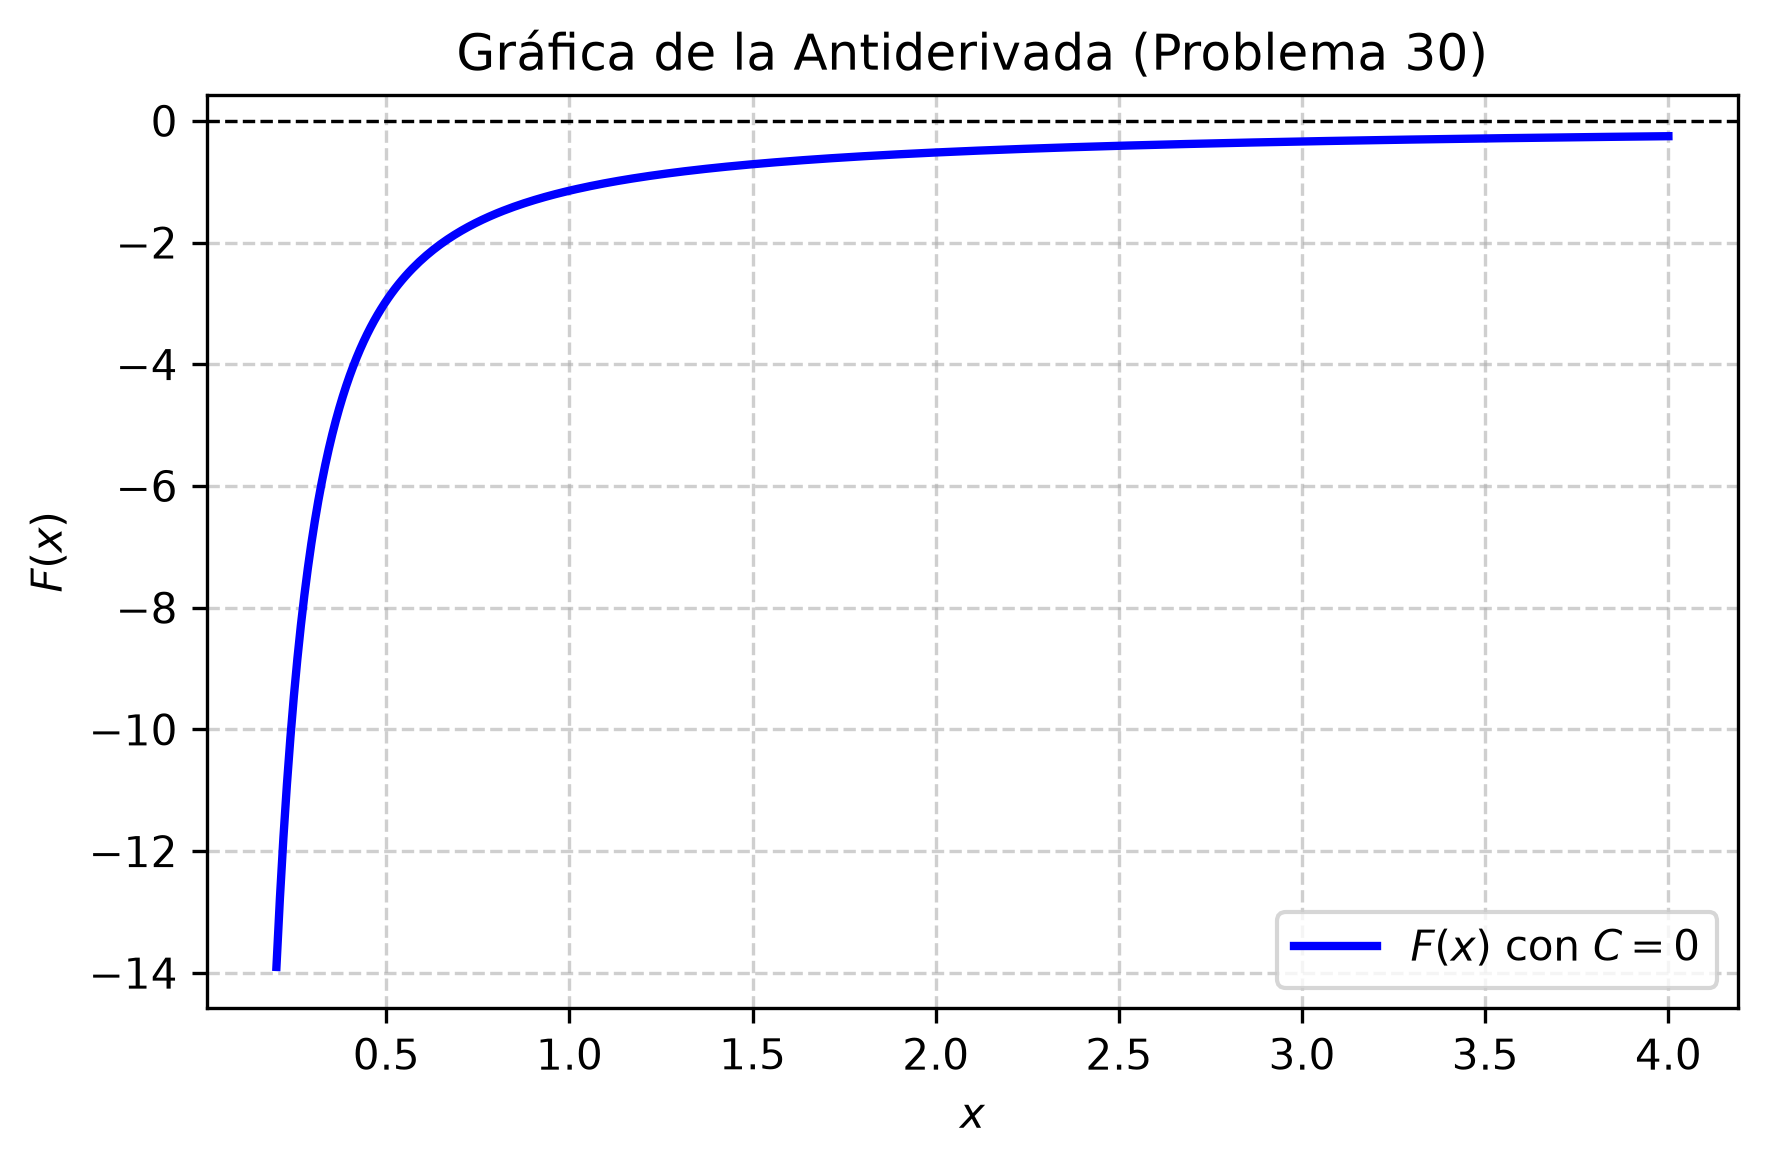
\includegraphics[width=\columnwidth]{semana_05/graficas/SEM05_P30_grafica.png}
	\caption{Representación gráfica de $f(x)$ y su antiderivada $F(x)$ evaluada para la constante de integración $C = 0$ (Problema 30).}
	\label{fig:problema30}
\end{figure}
